\documentclass{article}

\usepackage{tikz}
\usepackage{xcolor}
\usepackage{wrapfig}
\usepackage{hyperref}
\usepackage[margin=1in]{geometry}

\title{\textbf{Welcome to the Neuroidal Model\\ Research Group!}}
\author{Patrick Perrine, Mugizi Rwebangira}
\date{}

\begin{document}
 \maketitle

Hello and welcome to our group! This is meant to help onboard new members to our research, and also act as a reference packet for current members working on our project.

\section*{Who Are We?}

\begin{wrapfigure}{l}{0.35\textwidth}
    \centering
    \Large{Mugizi Rwebangira}\vspace{5mm}
    {%
	   \setlength{\fboxsep}{0pt}%
	   \setlength{\fboxrule}{3pt}%
	   \fbox{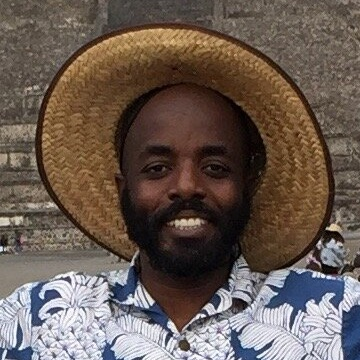
\includegraphics[width=0.3\textwidth]{pictures/mugizi_teotihuacan.jpeg}}%
	 }%
\end{wrapfigure} \hfill

I am a researcher in machine learning, artificial intelligence and computational neuroscience. I was born in Dar Es Salaam, Tanzania and got my Bachelors degree at Howard University in Washington, DC and my PhD at Carnegie Mellon in Pittsburgh, PA. Then I was a professor at Howard University where I taught algorithms, information theory and machine learning. Currently I am a professor at Calpoly San Luis Obispo.

I really think my most distinguishing characteristic has always been an insatiable curiosity. From an early age I remember always wanting to know as much as possible about (almost) everything. Hence, I became an academic. 

In my free time I really enjoy reading books, watching movies and running marathons (in that order). And of course I enjoy traveling (who doesn’t?). The picture on the left is from a trip to Mexico a few years ago.

\hfill \\

\begin{wrapfigure}{r}{0.35\textwidth}
    \centering
    \vspace{-6mm}\Large{Patrick Perrine}\vspace{5mm}
    {%
	   \setlength{\fboxsep}{0pt}%
	   \setlength{\fboxrule}{3pt}%
      \fbox{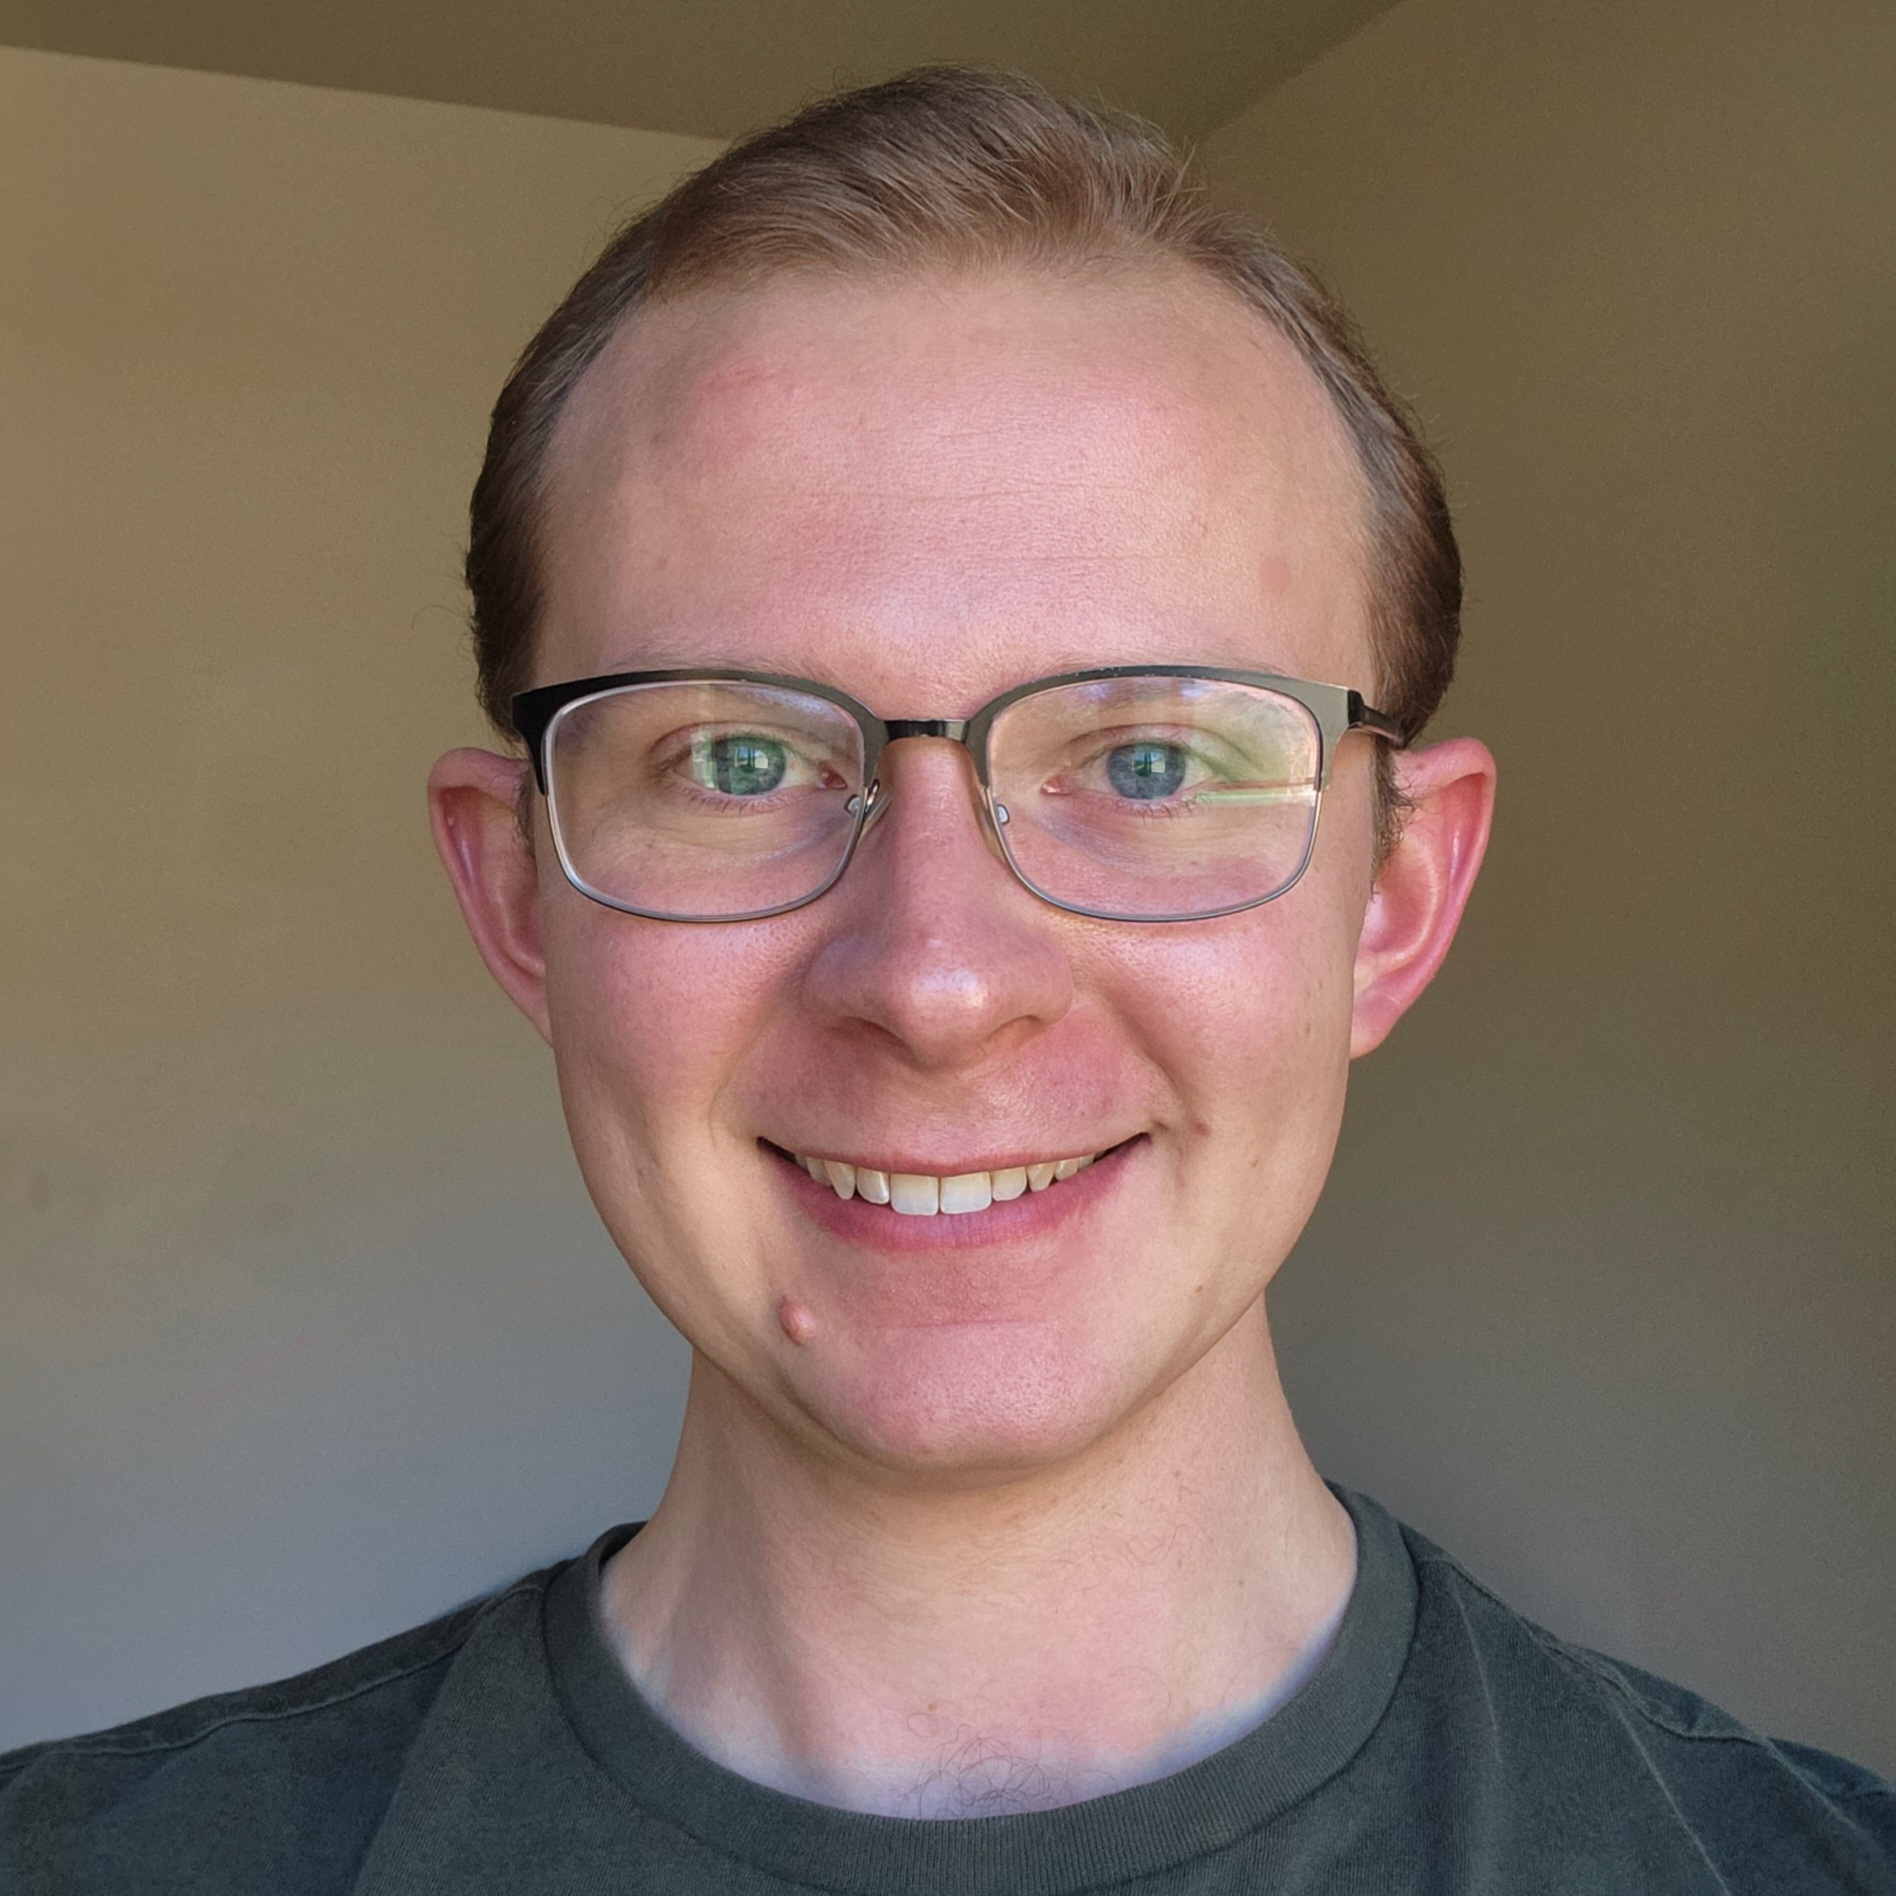
\includegraphics[width=0.3\textwidth]{pictures/patrick.jpg}}%
	 }%
\end{wrapfigure} \hfill

I am a machine learning researcher working remotely for Cal Poly in San Luis Obispo. I was born and raised in San Diego, CA, earned my B.S. in Computer Science at San Diego State University, and earned my M.S. in Computer Science at Cal Poly in June 2023. My current research interests lie in building foundational machine learning methods for interdisciplinary applications. 

My master’s thesis research consisted of an implementation of the Neuroidal model for use in unsupervised machine learning. Other previous research experience includes designing LSTM and GAN-based deep learning systems for interdisciplinary use such as human motion prediction/generation and image processing optimization. I have also taught a section of discrete mathematics at Cal Poly.

I enjoy swimming, taking my dog out on adventures, and listening to electronic music. I also like sharing my opinions about video games and movies with nerds on the internet.

\let\thefootnote\relax\footnotetext{Last Updated: \today}

%\newpage
%
%\begin{wrapfigure}{l}{0.35\textwidth}
%    \centering
%    \Large{Chandradeep Chowdhury}\vspace{5mm}
%    {%
%	   \setlength{\fboxsep}{0pt}%
%	   \setlength{\fboxrule}{3pt}%
%      \fbox{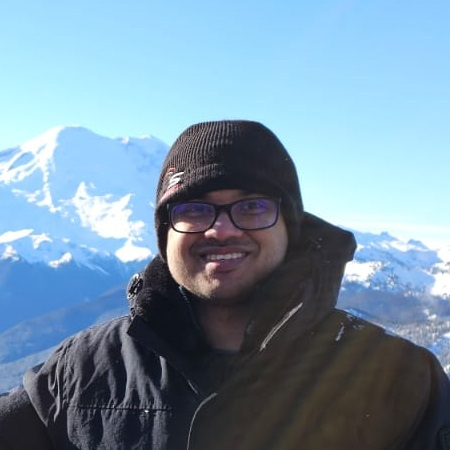
\includegraphics[width=0.3\textwidth]{pictures/chandradeep.jpg}}%
%	 }%
%\end{wrapfigure} \hfill
%
%\hfill \\
%
%\hfill \\
%
%I am a software engineer working on product recommendation systems. I have a BS in math and MS in computer science from Cal Poly. I currently stay in Seattle, WA. I like converting obscure theory into practical applications. My primary hobby is reading, writing, watching and critiquing science fiction novels and movies. My long term goal is to start my own company to sell edge automation devices for healthcare, agriculture and other industries.
%
%\hfill \\
%
%\hfill \\
%
%\begin{wrapfigure}{r}{0.35\textwidth}
%    \centering
%    \vspace{-2mm}\Large{Shosei Anegawa}\vspace{5mm}
%    {%
%	   \setlength{\fboxsep}{0pt}%
%	   \setlength{\fboxrule}{3pt}%
%      \fbox{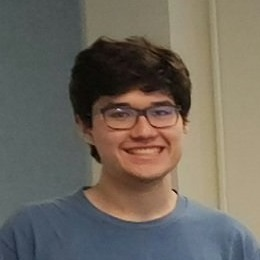
\includegraphics[width=0.3\textwidth]{pictures/shosei.jpg}}%
%	 }%
%\end{wrapfigure} \hfill
%
%\hfill \\
%
%\hfill \\
%
%I'm a 4th-year computer science major and math minor at Cal Poly. My research interests are largely in the field of machine learning, and most of my experience outside of this project is in computer vision and reinforcement learning. Outside of that, I really enjoy combinatorics. As for hobbies I enjoy playing video games (especially RPGs) and table top games (including but not limited to dungeons and dragons).
%
%\hfill \\
%
%\hfill \\
%
%\vspace{5cm}
%\begin{center}
%{\Large{More to arrive soon!}}
%\end{center}

\newpage

\section*{What Are We Working On?}

\hfill 

In simple terms, we are exploring a set of algorithms that exude realistic learning behaviors. We are investigating the \emph{Neuroidal Model}, which consists of a few procedures that allow a graph to gather information in a \textit{biologically plausible} manner. Other frameworks found within machine learning and artifical intelligence allow for highly performant learning, however, we argue that this model allows for a means to more closely model how humans learn into a machine. This project allows us to make fundamental contributions both within and outside of computer science. In the long run, we believe that this model will serve as a basis for a new wave of even more effective machine learning technologies. \\

We are using the following paper as the basis for our research, as it offers a wealth of insights as to how to use the Neuroidal model for effective and realistic learning: \\

\noindent \href{https://doi.org/10.1162/0899766053019890}{Leslie Valiant. Memorization and Association on a Realistic Neural Model. \textit{Neural Computation}, 2005.} \\

\noindent That paper describes a learning algorithm called ``JOIN,'' which is used to have a graph model (or ``brain'') memorize information in a biologically plausible manner. It is a rather dense paper, so it may take a few readings to fully understand. We have been building off of that paper in several ways, such as creating new algorithms, simulating the model using working code, and developing new mathematics to better understand all of the technical details. A guiding question for us in this project has been ``\textit{How much can the Neuroidal model possibly learn?}'' This interest has led us in many fruitful directions for the project. \\

All these efforts resulted in master's theses and senior projects from several students in the past two years. Using all our work, we published at the \href{https://2024.ccneuro.org/}{Cognitive Computational Neuroscience (CCN) Conference}! \\

\noindent 
\href{https://2024.ccneuro.org/poster/?id=585}{Patrick R. Perrine, Chandradeep Chowdhury, and Mugizi R. Rwebangira. Capacity of the Neuroidal Model for Shared Memory Representations. \textit{CCN}, Boston, August 2024.} \\

We are now aiming to have our continued work be compiled into an article under the Journal of Machine Learning Research (JMLR). We intend to model this paper similarly to this related workshop article: \\

\noindent 
\href{https://proceedings.mlr.press/v40/Papadimitriou15.html}{Christos Papadimitriou and Santosh Vempala. Cortical Learning via Prediction. In \textit{Conference on Learning Theory}, pp. 1402-1422. PMLR, 2015.} \\

Here are research milestones related to the Neuroidal model, with each referring to a published work:

\vspace{-2mm}

% For Research Milestone Table
\newcommand\ytl[2]{
\parbox[b]{8em}{\hfill{\color{black}\bfseries #1}~$\cdot\cdot\cdot\cdot\cdot$~}\makebox[0pt][c]{$\bullet$}\vrule\quad \parbox[c]{9cm}{\vspace{7pt}\color{black}\raggedright #2\\[7pt]}\\[-3pt]} 

\begin{table}[h]
\centering
\begin{minipage}[t]{1.\linewidth}
\color{red}
\rule{\linewidth}{1pt}
\ytl{1994}{``Circuits of the Mind'' Book Published}
%\ytl{2003}{Cell Assemblies Found in the Brain}
\ytl{2005}{JOIN Introduced with Replication Factor Relations \cite{valiant2005}}
\ytl{2006}{Findings of [2005] Comparable to Neuroscience Data}
\ytl{2008}{JOIN-like Memory Formation Observed in Human Brain}
\ytl{2009}{Neuroidal Circuits Industrially Simulated}
\ytl{2012}{Neuroidal Model Adapted to Act as Hippocampus}
\ytl{2015}{PJOIN Algorithm Introduced \cite{papadim2015}}
%\ytl{2017}{Capacity Analysis for Neuroidal Model Initiated}
\ytl{2020}{Assembly Calculus Introduced \cite{papadim2020}}
\ytl{2024}{We Published Our First Article! \cite{perrine2024}}
\bigskip
\rule{\linewidth}{1pt}%
\end{minipage}%
\end{table}

\newpage

%\noindent To end this section, here is how we like to describe the project in each of our own wording: \\
%
%\noindent ``Quote from Mugizi'' -- Mugizi \\
%``Quote from Patrick'' -- Patrick \\
%$\dots$

\section*{Where Are We Working?}

\begin{wrapfigure}{r}{0.3\textwidth}
    \centering
    %\vspace{-6mm}\Large{Patrick Perrine}\vspace{5mm}
    {%
	   \setlength{\fboxsep}{0pt}%
	   \setlength{\fboxrule}{0pt}%
      \fbox{
\includegraphics[width=0.2\textwidth]{pictures/teams.png}}%
	 }%
\end{wrapfigure} \hfill

We primarily work remotely using our Cal Poly license to Microsoft Teams. We utilize a main chat to discuss day-to-day updates and host weekly meetings with the whole group. We also meet in subgroups depending on the specific tasks that arise. Occasionally we have met in Mugizi's office when possible, but people's schedules can often end up being in flux with one another. For example, Patrick is back in San Diego and Chandradeep Chowdhury is currently in Seattle, so they unfortunately will have to contribute virtually!

\section*{Why Are We Working On This?}

\hfill

Because it is interesting! But more specifically, we have all expressed a great interest in machine learning, and we feel this is the best way we can contribute to this huge space within artificial intelligence. Also, we all seem to enjoy learning from other disciplines whether it be from mathematics, neuroscience, or other forms of engineering, so we have been able to take insights from other fields to strengthen our work in this project. \\

Some of us also have specific career goals, such as obtaining funding for the project after publication, entering a Ph.D. program to continue similar work, and/or advancing within industry using the expert knowledge demonstrated here. As we've continued to work on this project for the past year and a half, we have all found it to be both academically and professionally valuable to us.

\section*{How Are We Working On The Neuroidal Model?}

Using the 2005 paper as our primary source of inspiration, we have done several things to build off of the Neuroidal model. Here is an abridged version of some of our milestones:

\begin{itemize}
\item[$\cdot$]Mugizi surveyed attendees of CCN 2022 to see whether other researchers would find additions to the Neuroidal model interesting, with positive results.
\item[$\cdot$]Patrick completed his thesis based on the simulation of the Neuroidal model, along with creating a new algorithm ``QJOIN'' to significantly speed up memorization within the model \cite{perrine2023}.
\item[$\cdot$]Chandradeep Chowdhury completed his thesis based on a theoretical framework for investigating instances of interference within the model, which is a crucial metric for measuring capacity \cite{chowdhury2023}.
\item[$\cdot$]Shosei Anegawa helped us to interpret the theoretical foundations of the model, while also applying deep learning to optimize parameters for the Neuroidal model.
\item[$\cdot$]Eben Sherwood created and implemented a new algorithm, SeqMem, in order to meaningfully store temporal information within the model \cite{sherwood2024}.
\item[$\cdot$]Ethan Wolfe implemented new type of graph structure to work with the model, known as ``Small-Worlds,'' which affected the efficiency and the biological plausibility of our approach \cite{wolfe2024}.
\item[$\cdot$]Yanna Shirokova improved the underlying simulation procedure drastically by using GPU-accelerated code, and then ran tests on an industrial supercomputer.
\item[$\cdot$]Arthur Umerov performed rigorous numerical calculations in a manner similar to the 2005 paper, helping us to find better parameters for the model that hold true to its original formulation.
\end{itemize}

\newpage

\section*{How Can You Contribute?}

We are so glad that you asked!

\begin{itemize}
\item[$\cdot$]Attend our weekly meetings!
\item[$\cdot$]Read the related work for our project.
\item[$\cdot$]Brainstorm ideas on how we can add to or improve the model.
\item[$\cdot$]Contribute to our codebase hosted here: \url{https://github.com/chandradeep24/Valiant}
\end{itemize} 

\noindent We are rather open to feedback as to how we may better our methods. Given how theoretical this whole project is in spirit, we are still in a sort of ``ideation'' phase, as opposed to maintaining a rigid engineering pipeline for producing work. Please offer any perspective you may have in our meetings or with us individually. Also, here are some useful links to papers that will definitely come in handy when working on the project: \\

\vspace{4mm}
\noindent{\Large{\textbf{Required Reading}}}

\renewcommand{\section}[2]{}

\begin{thebibliography}{1}
\bibitem{perrine2024}
Patrick R. Perrine, Chandradeep Chowdhury, and Mugizi R. Rwebangira. Capacity of the Neuroidal Model for Shared Memory Representations. \textit{Conference on Cognitive Computational Neuroscience}, Boston, August 2024. \url{https://2024.ccneuro.org/poster/?id=585}
\end{thebibliography}

\vspace{4mm}
\noindent{\Large{\textbf{Related Reading}}}

\begin{thebibliography}{9}
\makeatletter
\addtocounter{\@listctr}{1}
\makeatother

\bibitem{valiant2005}
Leslie G. Valiant. Memorization and Association on a Realistic Neural Model. \textit{Neural Computation}, 17(3):527–555, 2005. \url{https://doi.org/10.1162/0899766053019890}

\bibitem{perrine2023}
Patrick R. Perrine. Neural Tabula Rasa: Foundations for Realistic Memories and Learning. Master’s thesis, California Polytechnic State University, San Luis Obispo, June 2023. \url{https://digitalcommons.calpoly.edu/theses/2782}

\bibitem{chowdhury2023}
Chandradeep Chowdhury. Foundations Of Memory Capacity In Models Of Neural Cognition. Master’s thesis, California Polytechnic State University, San Luis Obispo, December 2023. \url{https://digitalcommons.calpoly.edu/theses/2718}

\bibitem{sherwood2024}
Eben M. Sherwood. Sequential Memory Generation for Cognitive Models. Master’s thesis, California Polytechnic State University, San Luis Obispo, June 2024. \url{https://digitalcommons.calpoly.edu/theses/2849}%2859

\bibitem{wolfe2024}
Ethan I. Wolfe. The Effect of Watts-Strogatz and Barabasi-Albert graphs on Memory Formation. Master’s thesis, California Polytechnic State University, San Luis Obispo, June 2024. \url{https://digitalcommons.calpoly.edu/theses/2859}%

\bibitem{papadim2015}
Christos H. Papadimitriou and Santosh S. Vempala. Cortical Learning via Prediction. In \textit{Conference on Learning Theory}, pp. 1402-1422. PMLR, 2015. \url{https://proceedings.mlr.press/v40/Papadimitriou15.html}

\bibitem{papadim2020}
Christos H. Papadimitriou, Santosh S. Vempala, Daniel Mitropolsky, Michael Collins, and Wolfgang Maass. Brain Computation by Assemblies of Neurons. Proceedings of the National Academy of Sciences 117, no. 25 (2020): 14464-14472. \url{https://doi.org/10.1073/pnas.2001893117}

%\bibitem{valiant1994}
%Leslie G. Valiant. \textit{Circuits of the Mind}. New York, NY, 1994, 2000. \url{https://global.oup.com/academic/product/circuits-of-the-mind-9780195126686}

%\bibitem{valiant2017}
%Leslie G. Valiant. Capacity of Neural Networks for Lifelong Learning of Composable Tasks. In \textit{Proceedings of the Symposium on Foundations of Computer Science (FOCS)}, pages 367–378, Berkeley, 2017. IEEE. \url{https://doi.org/10.1109/FOCS.2017.41}
\end{thebibliography} 

\vspace{1.5cm}
\begin{center}
{\Large{We hope to hear from you soon!}}
\end{center}

\end{document}